\documentclass[11pt]{article}
\usepackage[textwidth=18.0cm, textheight=23.0cm, top=2.0cm]{geometry}
\usepackage{pst-all}
\usepackage{amssymb}
\usepackage{tikz}
\usepackage{underscore}\begin{document}
\pagestyle{empty}


ClassName: \underline{\textbf{Class_10.2bp-22}}
\par
BinSize: \underline{\textbf{100 × 100}}
\par
ReduceSize: \underline{\textbf{100 × 100}}
\par
TypeNum: \underline{\textbf{60}}
\par
Num: \underline{\textbf{60}}
\par
OutS: \underline{\textbf{110000}}
\par
InS: \underline{\textbf{102593}}
\par
Rate: \underline{\textbf{0.933}}
\par
UB: \underline{\textbf{11}}
\par
LB0: \underline{\textbf{11}}
\par
LB: \underline{\textbf{11}}
\par
LBWithCut: \underline{\textbf{11}}
\par
NodeCut: \underline{\textbf{0}}
\par
ExtendedNodeCnt: \underline{\textbf{1}}
\par
GenNodeCnt: \underline{\textbf{1}}
\par
PrimalNode: \underline{\textbf{0}}
\par
ColumnCount: \underline{\textbf{11}}
\par
TotalCutCount: \underline{\textbf{0}}
\par
RootCutCount: \underline{\textbf{0}}
\par
LPSolverCnt: \underline{\textbf{1}}
\par
PricingSolverCnt: \underline{\textbf{0}}
\par
BranchAndBoundNum: \underline{\textbf{1}}
\par
isOpt: \underline{\textbf{true}}
\par
TimeOnInitSolution: \underline{\textbf{600.000 s}}
\par
TimeOnPrimal: \underline{\textbf{0.000 s}}
\par
TimeOnPricing: \underline{\textbf{0.000 s}}
\par
TimeOnRmp: \underline{\textbf{0.063 s}}
\par
TotalTime: \underline{\textbf{600.344 s}}
\par
\newpage


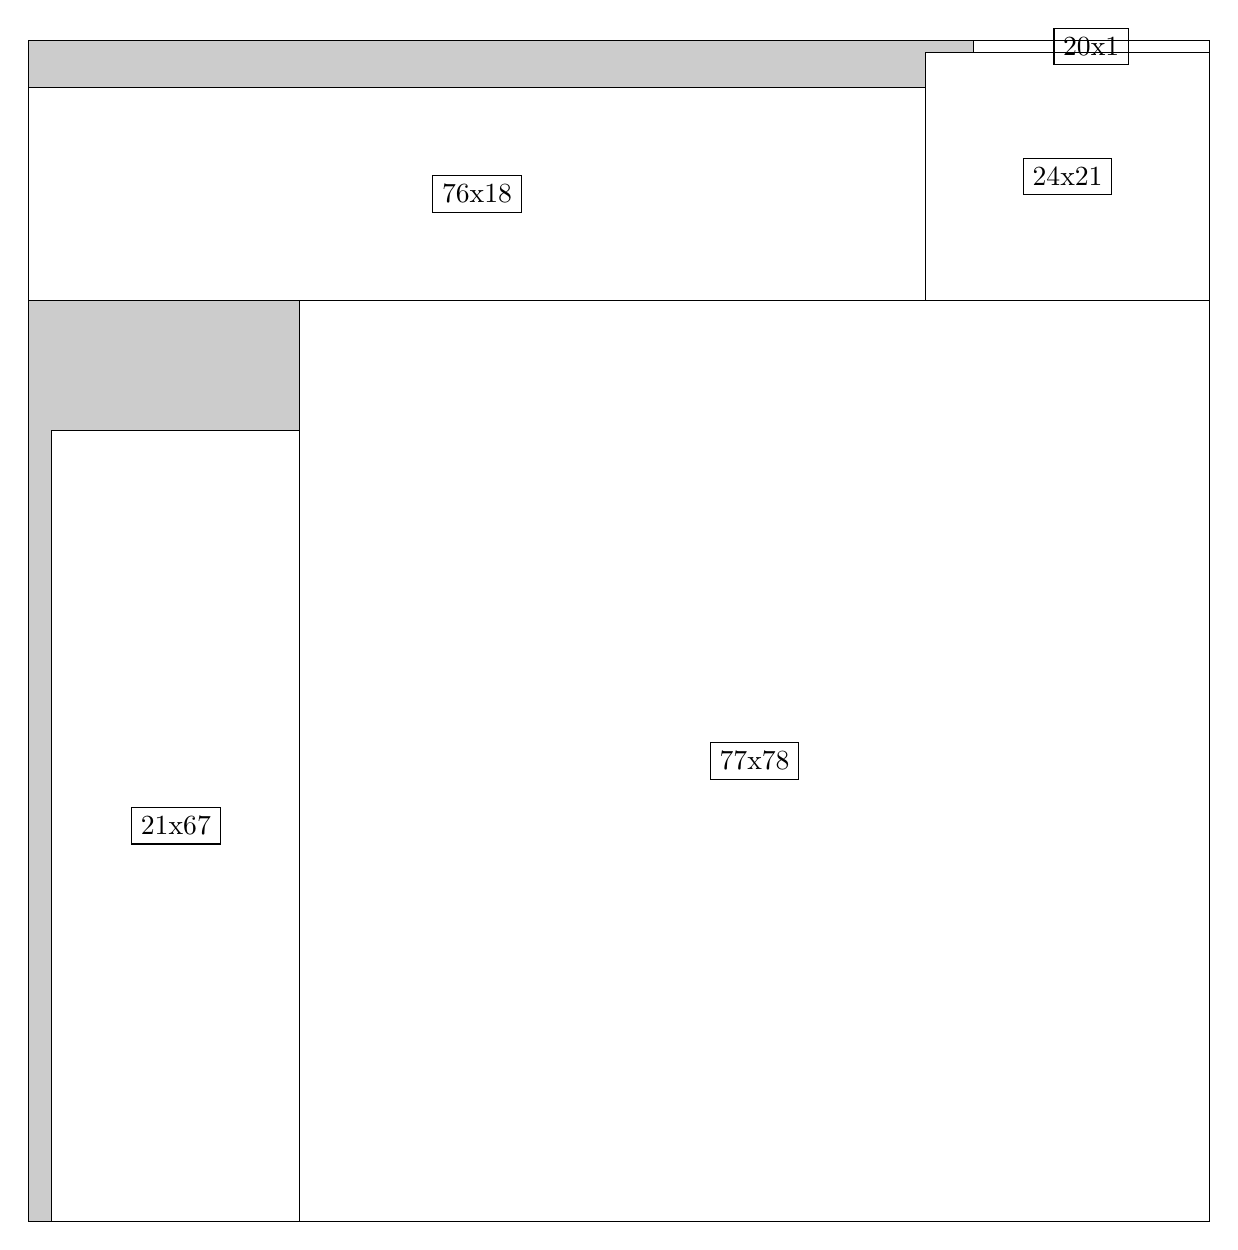
\begin{tikzpicture}[shorten >=1pt,scale=1.0,every node/.style={scale=1.0},->]
\tikzstyle{vertex}=[circle,fill=black!25,minimum size=14pt,inner sep=0pt]
\filldraw[fill=gray!40!white, draw=black] (0,0) rectangle (15.0,15.0);
\foreach \name/\x/\y/\w/\h in {77x78/3.4499999999999997/0.0/11.549999999999999/11.7,21x67/0.3/0.0/3.15/10.049999999999999,24x21/11.4/11.7/3.5999999999999996/3.15,20x1/12.0/14.85/3.0/0.15,76x18/0.0/11.7/11.4/2.6999999999999997}
\filldraw[fill=white!40!white, draw=black] (\x,\y) rectangle node[draw] (\name) {\name} ++(\w,\h);
\end{tikzpicture}


w =77 , h =78 , x =23 , y =0 , v =6006
\par
w =21 , h =67 , x =2 , y =0 , v =1407
\par
w =24 , h =21 , x =76 , y =78 , v =504
\par
w =20 , h =1 , x =80 , y =99 , v =20
\par
w =76 , h =18 , x =0 , y =78 , v =1368
\par
\newpage


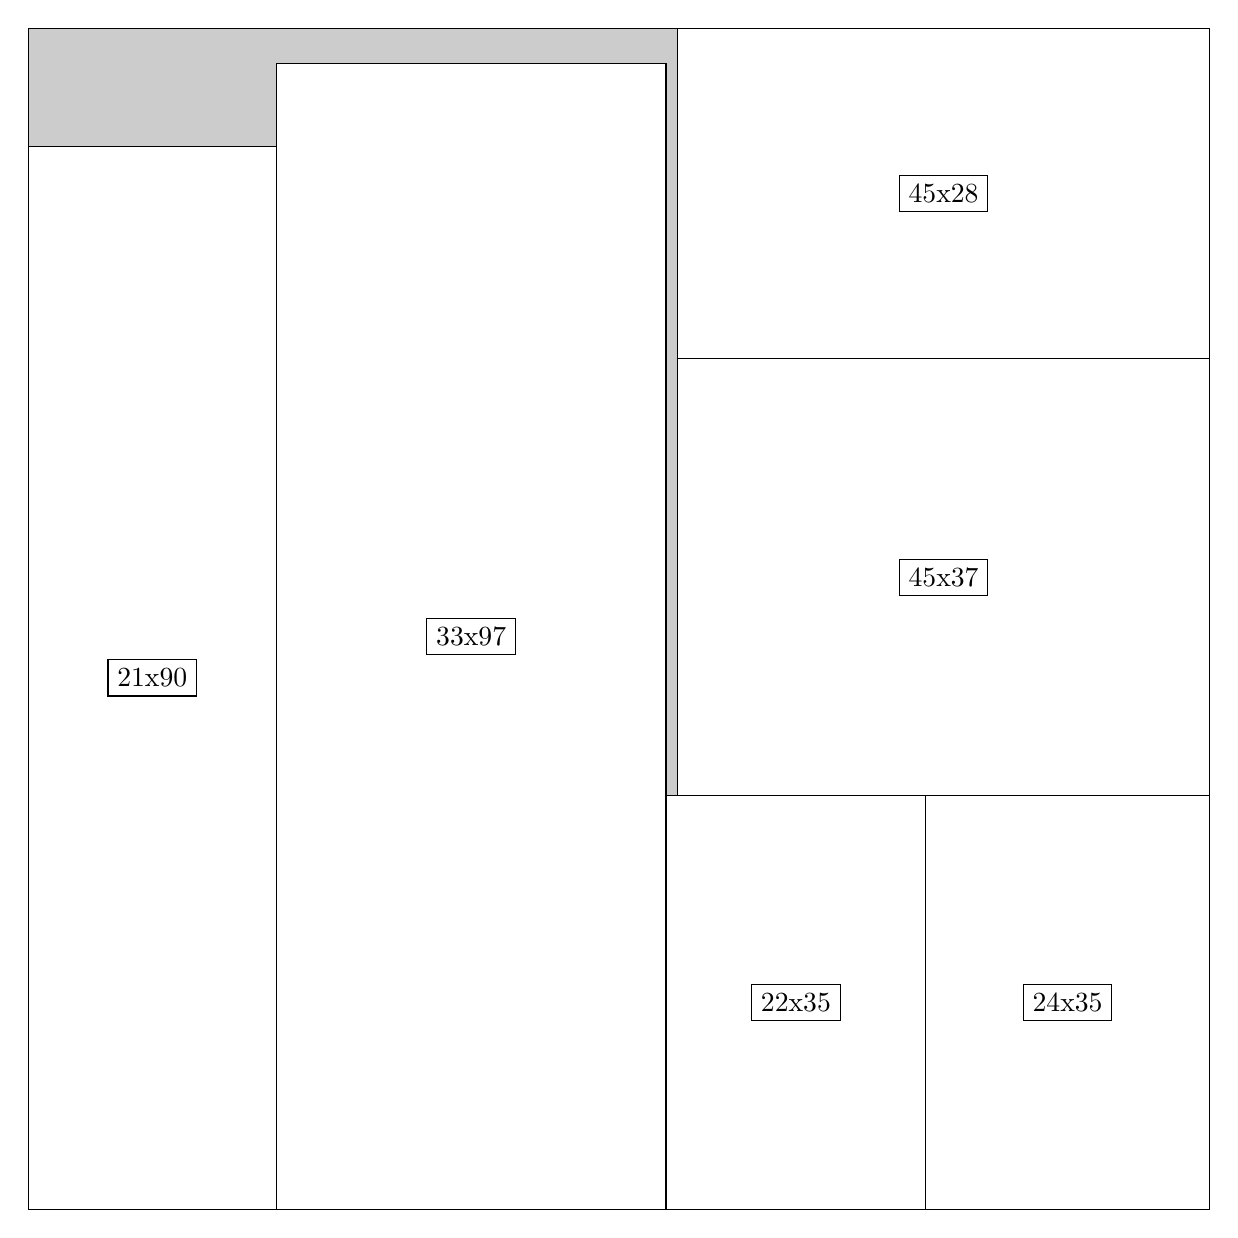
\begin{tikzpicture}[shorten >=1pt,scale=1.0,every node/.style={scale=1.0},->]
\tikzstyle{vertex}=[circle,fill=black!25,minimum size=14pt,inner sep=0pt]
\filldraw[fill=gray!40!white, draw=black] (0,0) rectangle (15.0,15.0);
\foreach \name/\x/\y/\w/\h in {24x35/11.4/0.0/3.5999999999999996/5.25,22x35/8.1/0.0/3.3/5.25,45x37/8.25/5.25/6.75/5.55,45x28/8.25/10.799999999999999/6.75/4.2,33x97/3.15/0.0/4.95/14.549999999999999,21x90/0.0/0.0/3.15/13.5}
\filldraw[fill=white!40!white, draw=black] (\x,\y) rectangle node[draw] (\name) {\name} ++(\w,\h);
\end{tikzpicture}


w =24 , h =35 , x =76 , y =0 , v =840
\par
w =22 , h =35 , x =54 , y =0 , v =770
\par
w =45 , h =37 , x =55 , y =35 , v =1665
\par
w =45 , h =28 , x =55 , y =72 , v =1260
\par
w =33 , h =97 , x =21 , y =0 , v =3201
\par
w =21 , h =90 , x =0 , y =0 , v =1890
\par
\newpage


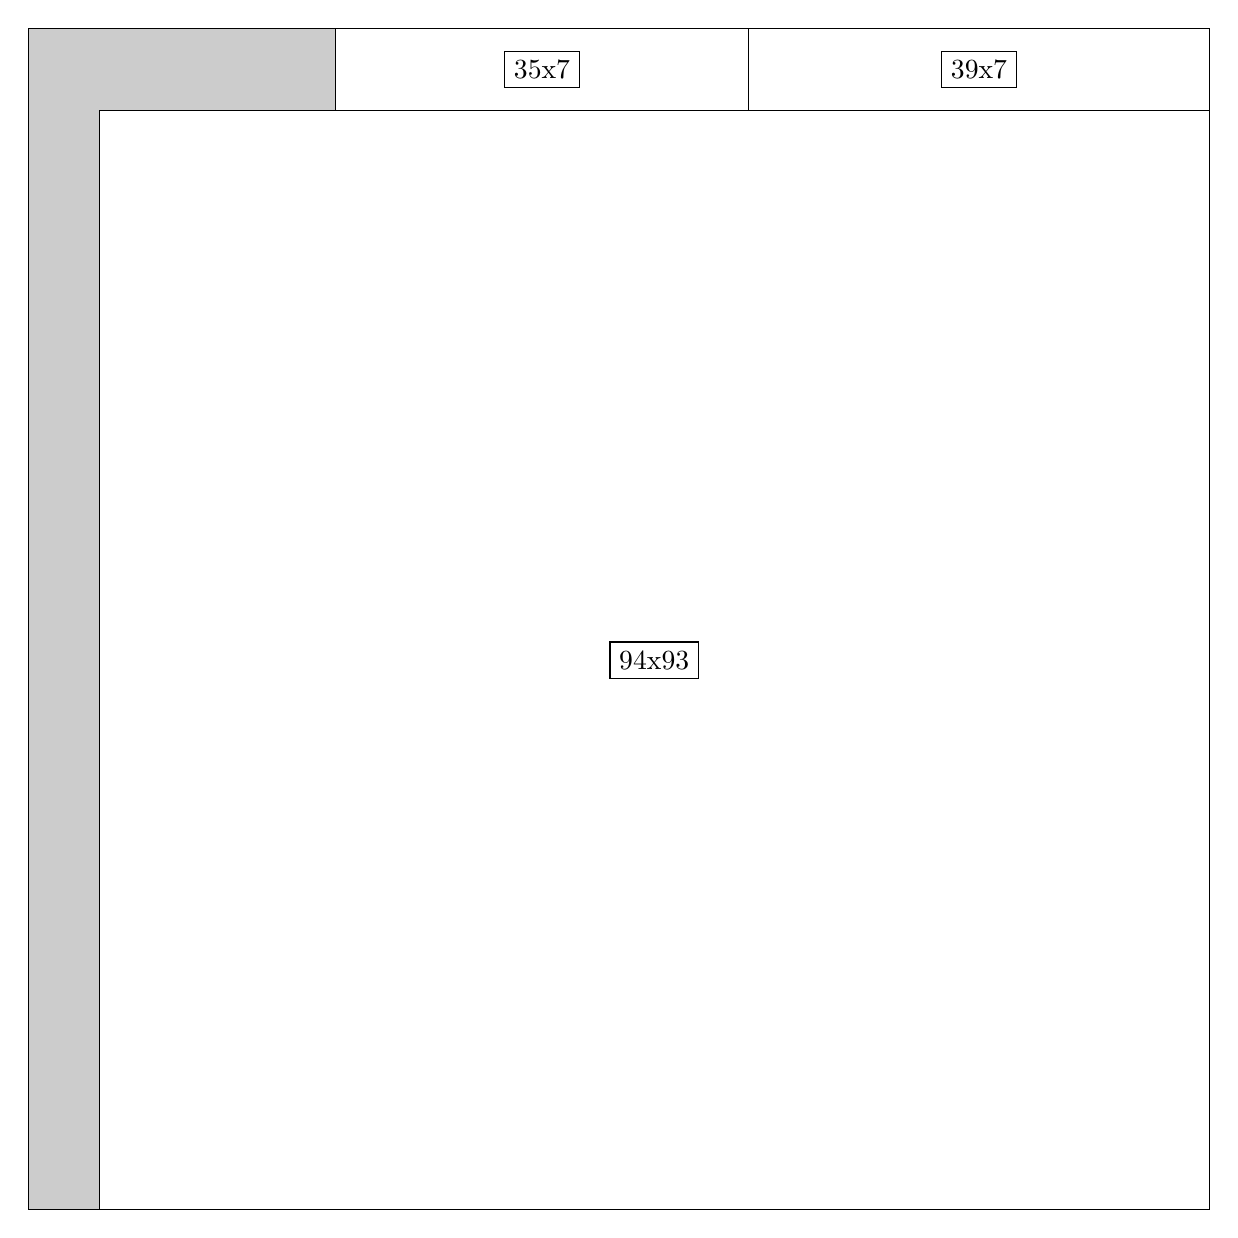
\begin{tikzpicture}[shorten >=1pt,scale=1.0,every node/.style={scale=1.0},->]
\tikzstyle{vertex}=[circle,fill=black!25,minimum size=14pt,inner sep=0pt]
\filldraw[fill=gray!40!white, draw=black] (0,0) rectangle (15.0,15.0);
\foreach \name/\x/\y/\w/\h in {94x93/0.8999999999999999/0.0/14.1/13.95,39x7/9.15/13.95/5.85/1.05,35x7/3.9/13.95/5.25/1.05}
\filldraw[fill=white!40!white, draw=black] (\x,\y) rectangle node[draw] (\name) {\name} ++(\w,\h);
\end{tikzpicture}


w =94 , h =93 , x =6 , y =0 , v =8742
\par
w =39 , h =7 , x =61 , y =93 , v =273
\par
w =35 , h =7 , x =26 , y =93 , v =245
\par
\newpage


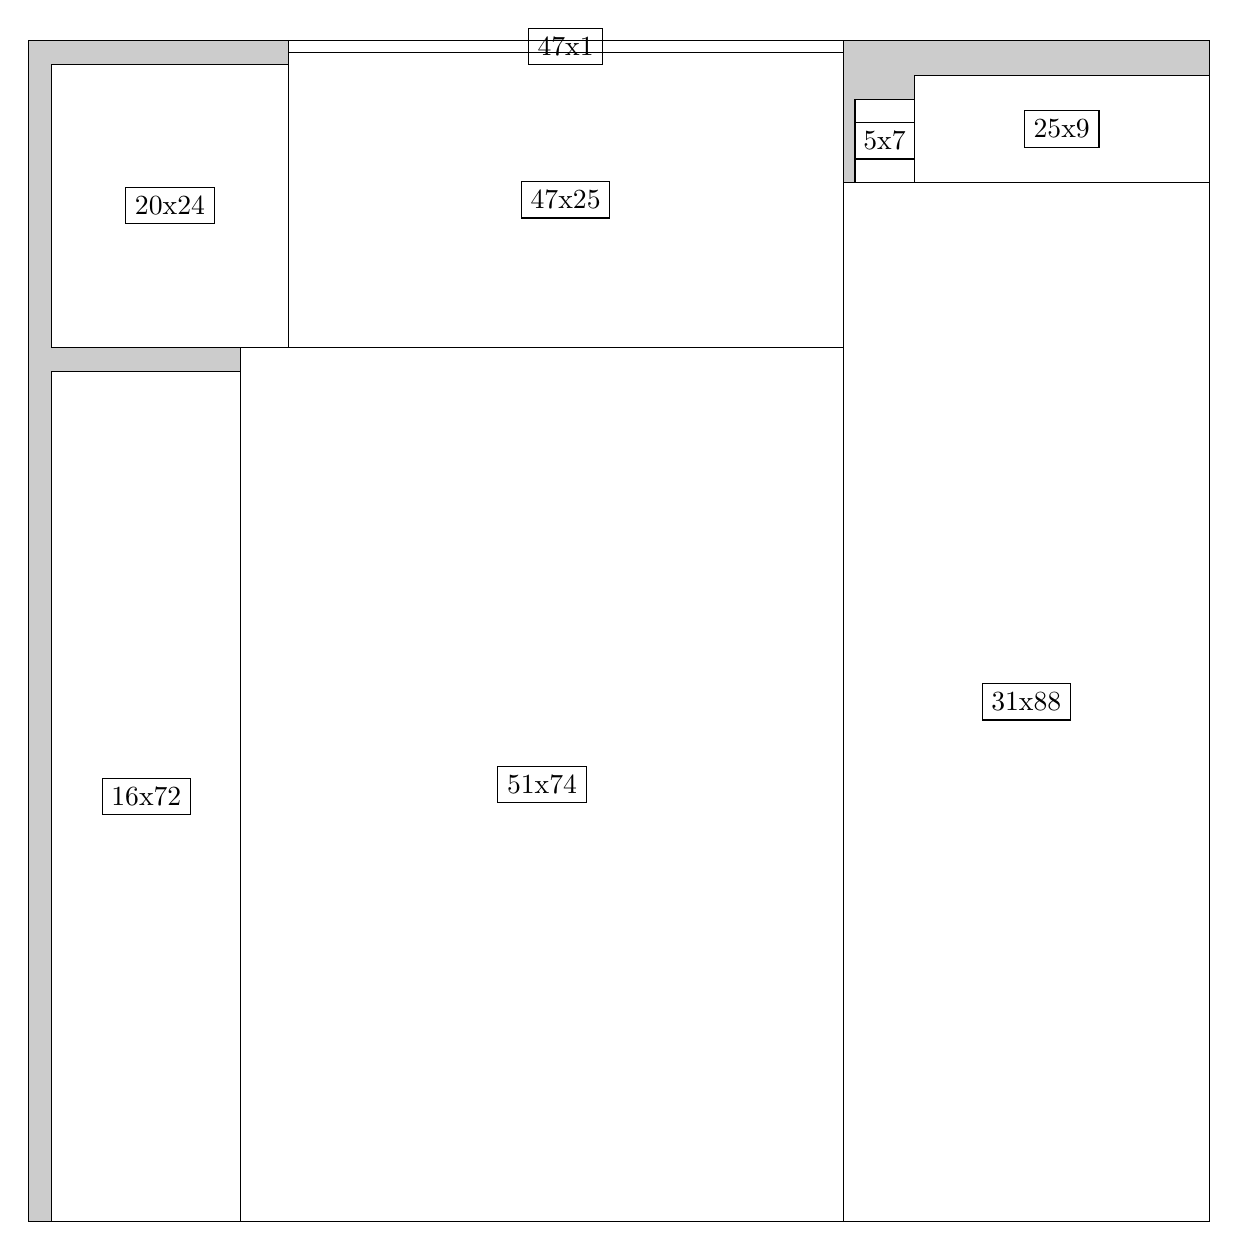
\begin{tikzpicture}[shorten >=1pt,scale=1.0,every node/.style={scale=1.0},->]
\tikzstyle{vertex}=[circle,fill=black!25,minimum size=14pt,inner sep=0pt]
\filldraw[fill=gray!40!white, draw=black] (0,0) rectangle (15.0,15.0);
\foreach \name/\x/\y/\w/\h in {31x88/10.35/0.0/4.6499999999999995/13.2,25x9/11.25/13.2/3.75/1.3499999999999999,5x7/10.5/13.2/0.75/1.05,51x74/2.6999999999999997/0.0/7.6499999999999995/11.1,16x72/0.3/0.0/2.4/10.799999999999999,47x25/3.3/11.1/7.05/3.75,47x1/3.3/14.85/7.05/0.15,20x24/0.3/11.1/3.0/3.5999999999999996}
\filldraw[fill=white!40!white, draw=black] (\x,\y) rectangle node[draw] (\name) {\name} ++(\w,\h);
\end{tikzpicture}


w =31 , h =88 , x =69 , y =0 , v =2728
\par
w =25 , h =9 , x =75 , y =88 , v =225
\par
w =5 , h =7 , x =70 , y =88 , v =35
\par
w =51 , h =74 , x =18 , y =0 , v =3774
\par
w =16 , h =72 , x =2 , y =0 , v =1152
\par
w =47 , h =25 , x =22 , y =74 , v =1175
\par
w =47 , h =1 , x =22 , y =99 , v =47
\par
w =20 , h =24 , x =2 , y =74 , v =480
\par
\newpage


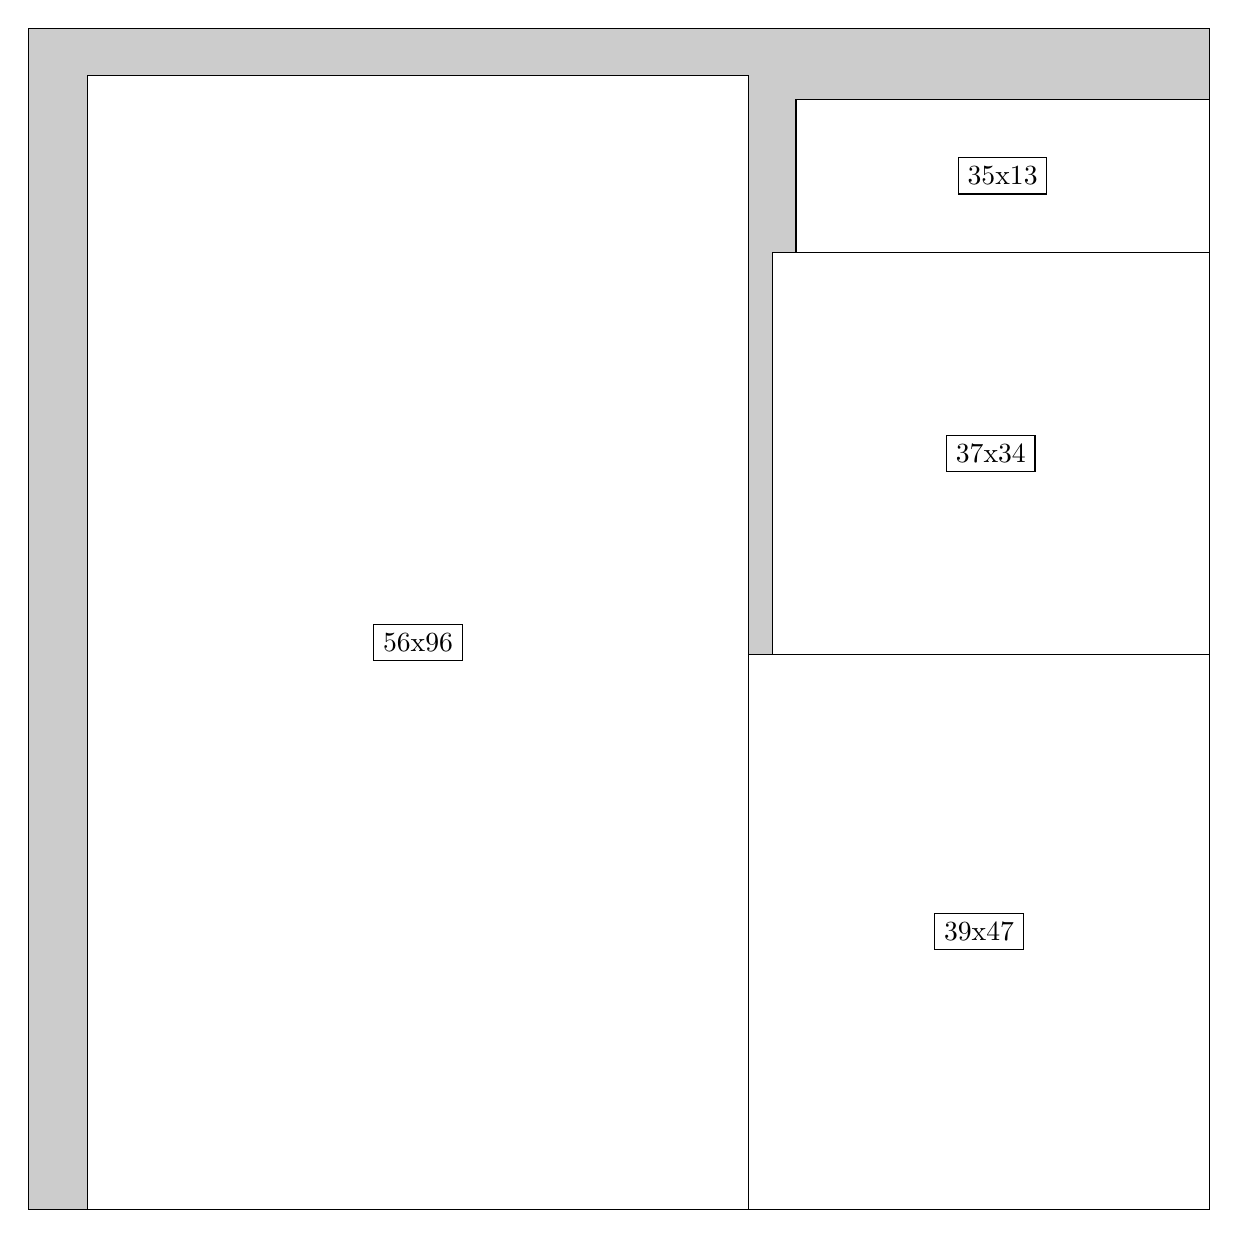
\begin{tikzpicture}[shorten >=1pt,scale=1.0,every node/.style={scale=1.0},->]
\tikzstyle{vertex}=[circle,fill=black!25,minimum size=14pt,inner sep=0pt]
\filldraw[fill=gray!40!white, draw=black] (0,0) rectangle (15.0,15.0);
\foreach \name/\x/\y/\w/\h in {39x47/9.15/0.0/5.85/7.05,37x34/9.45/7.05/5.55/5.1,35x13/9.75/12.15/5.25/1.95,56x96/0.75/0.0/8.4/14.399999999999999}
\filldraw[fill=white!40!white, draw=black] (\x,\y) rectangle node[draw] (\name) {\name} ++(\w,\h);
\end{tikzpicture}


w =39 , h =47 , x =61 , y =0 , v =1833
\par
w =37 , h =34 , x =63 , y =47 , v =1258
\par
w =35 , h =13 , x =65 , y =81 , v =455
\par
w =56 , h =96 , x =5 , y =0 , v =5376
\par
\newpage


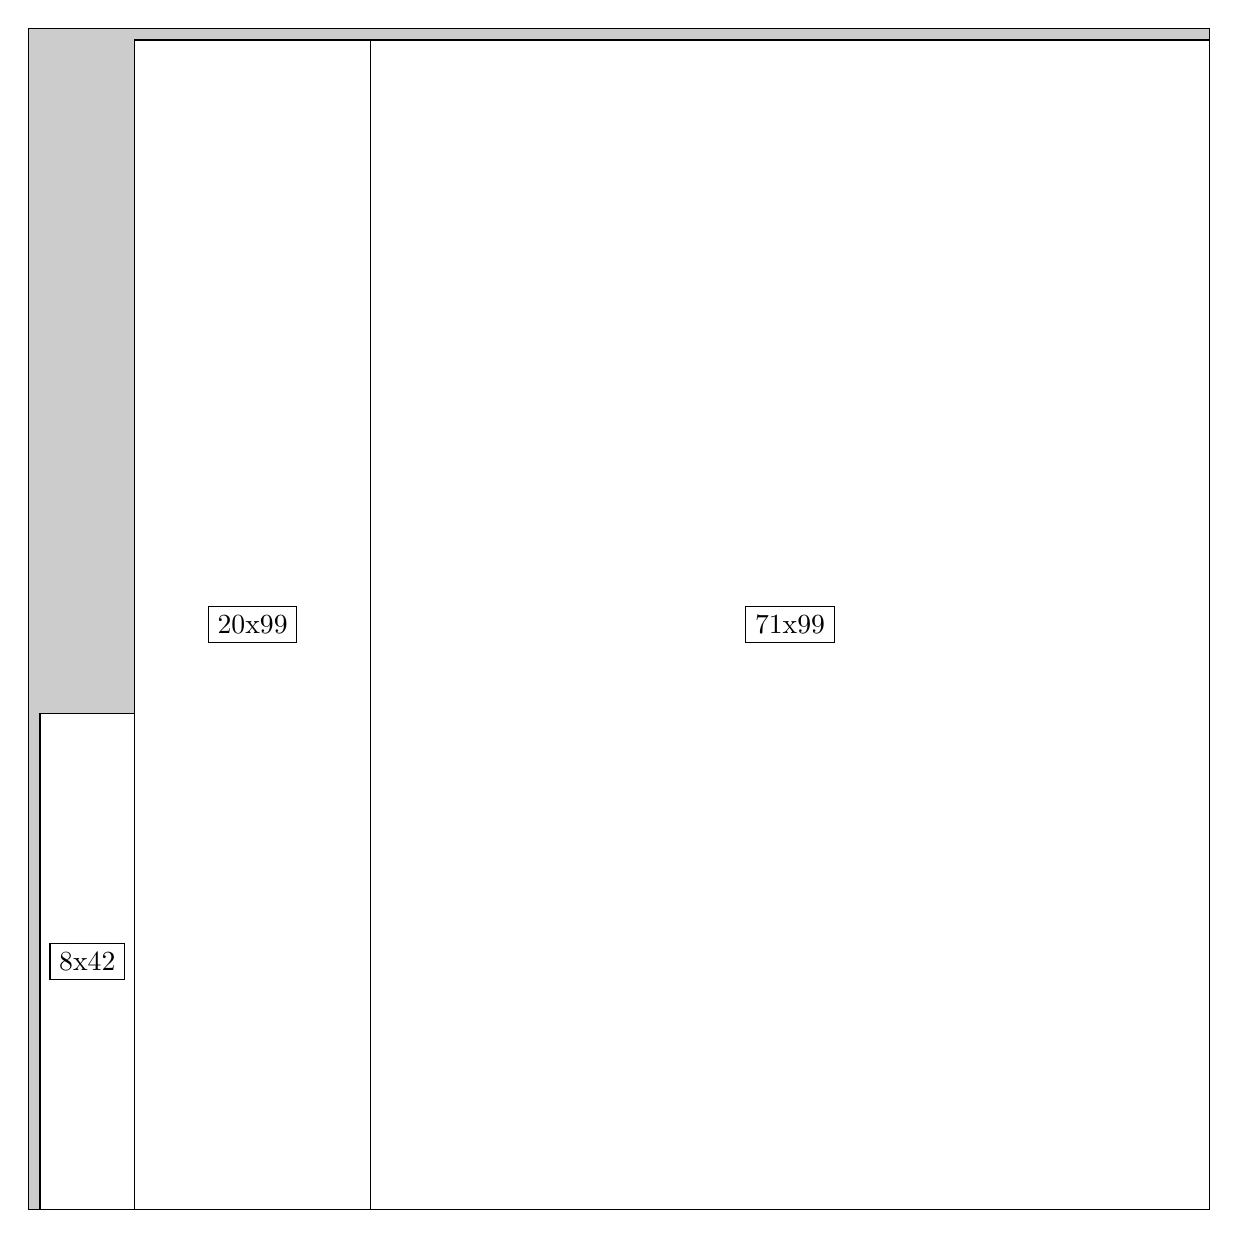
\begin{tikzpicture}[shorten >=1pt,scale=1.0,every node/.style={scale=1.0},->]
\tikzstyle{vertex}=[circle,fill=black!25,minimum size=14pt,inner sep=0pt]
\filldraw[fill=gray!40!white, draw=black] (0,0) rectangle (15.0,15.0);
\foreach \name/\x/\y/\w/\h in {71x99/4.35/0.0/10.65/14.85,20x99/1.3499999999999999/0.0/3.0/14.85,8x42/0.15/0.0/1.2/6.3}
\filldraw[fill=white!40!white, draw=black] (\x,\y) rectangle node[draw] (\name) {\name} ++(\w,\h);
\end{tikzpicture}


w =71 , h =99 , x =29 , y =0 , v =7029
\par
w =20 , h =99 , x =9 , y =0 , v =1980
\par
w =8 , h =42 , x =1 , y =0 , v =336
\par
\newpage


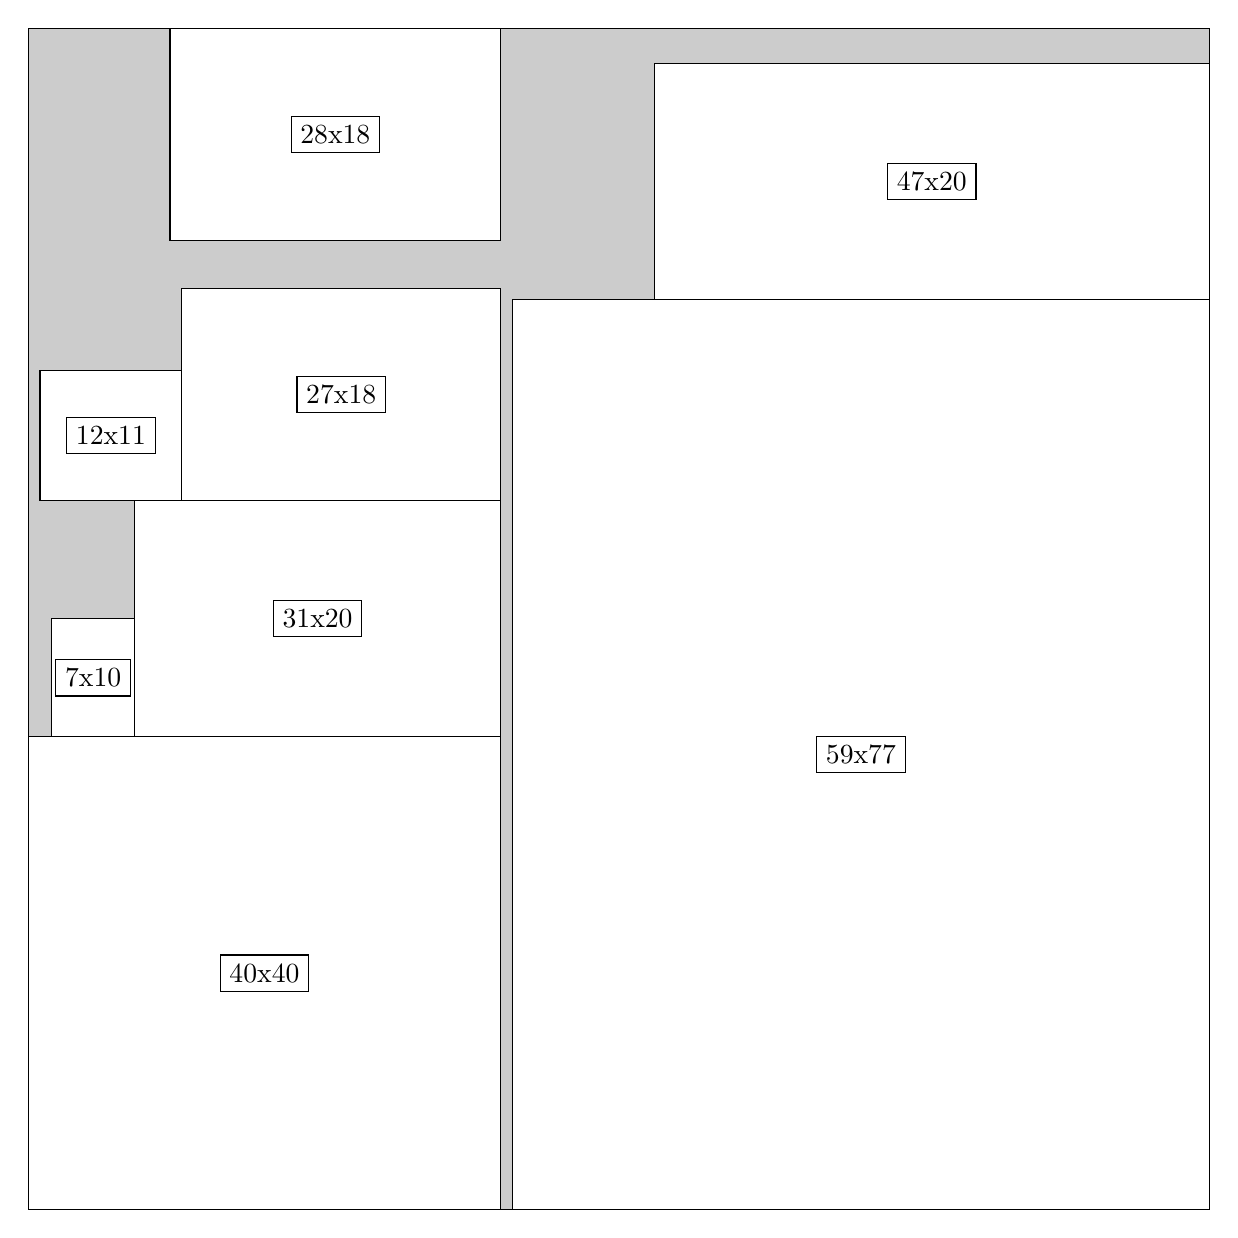
\begin{tikzpicture}[shorten >=1pt,scale=1.0,every node/.style={scale=1.0},->]
\tikzstyle{vertex}=[circle,fill=black!25,minimum size=14pt,inner sep=0pt]
\filldraw[fill=gray!40!white, draw=black] (0,0) rectangle (15.0,15.0);
\foreach \name/\x/\y/\w/\h in {59x77/6.1499999999999995/0.0/8.85/11.549999999999999,47x20/7.949999999999999/11.549999999999999/7.05/3.0,40x40/0.0/0.0/6.0/6.0,31x20/1.3499999999999999/6.0/4.6499999999999995/3.0,7x10/0.3/6.0/1.05/1.5,27x18/1.95/9.0/4.05/2.6999999999999997,12x11/0.15/9.0/1.7999999999999998/1.65,28x18/1.7999999999999998/12.299999999999999/4.2/2.6999999999999997}
\filldraw[fill=white!40!white, draw=black] (\x,\y) rectangle node[draw] (\name) {\name} ++(\w,\h);
\end{tikzpicture}


w =59 , h =77 , x =41 , y =0 , v =4543
\par
w =47 , h =20 , x =53 , y =77 , v =940
\par
w =40 , h =40 , x =0 , y =0 , v =1600
\par
w =31 , h =20 , x =9 , y =40 , v =620
\par
w =7 , h =10 , x =2 , y =40 , v =70
\par
w =27 , h =18 , x =13 , y =60 , v =486
\par
w =12 , h =11 , x =1 , y =60 , v =132
\par
w =28 , h =18 , x =12 , y =82 , v =504
\par
\newpage


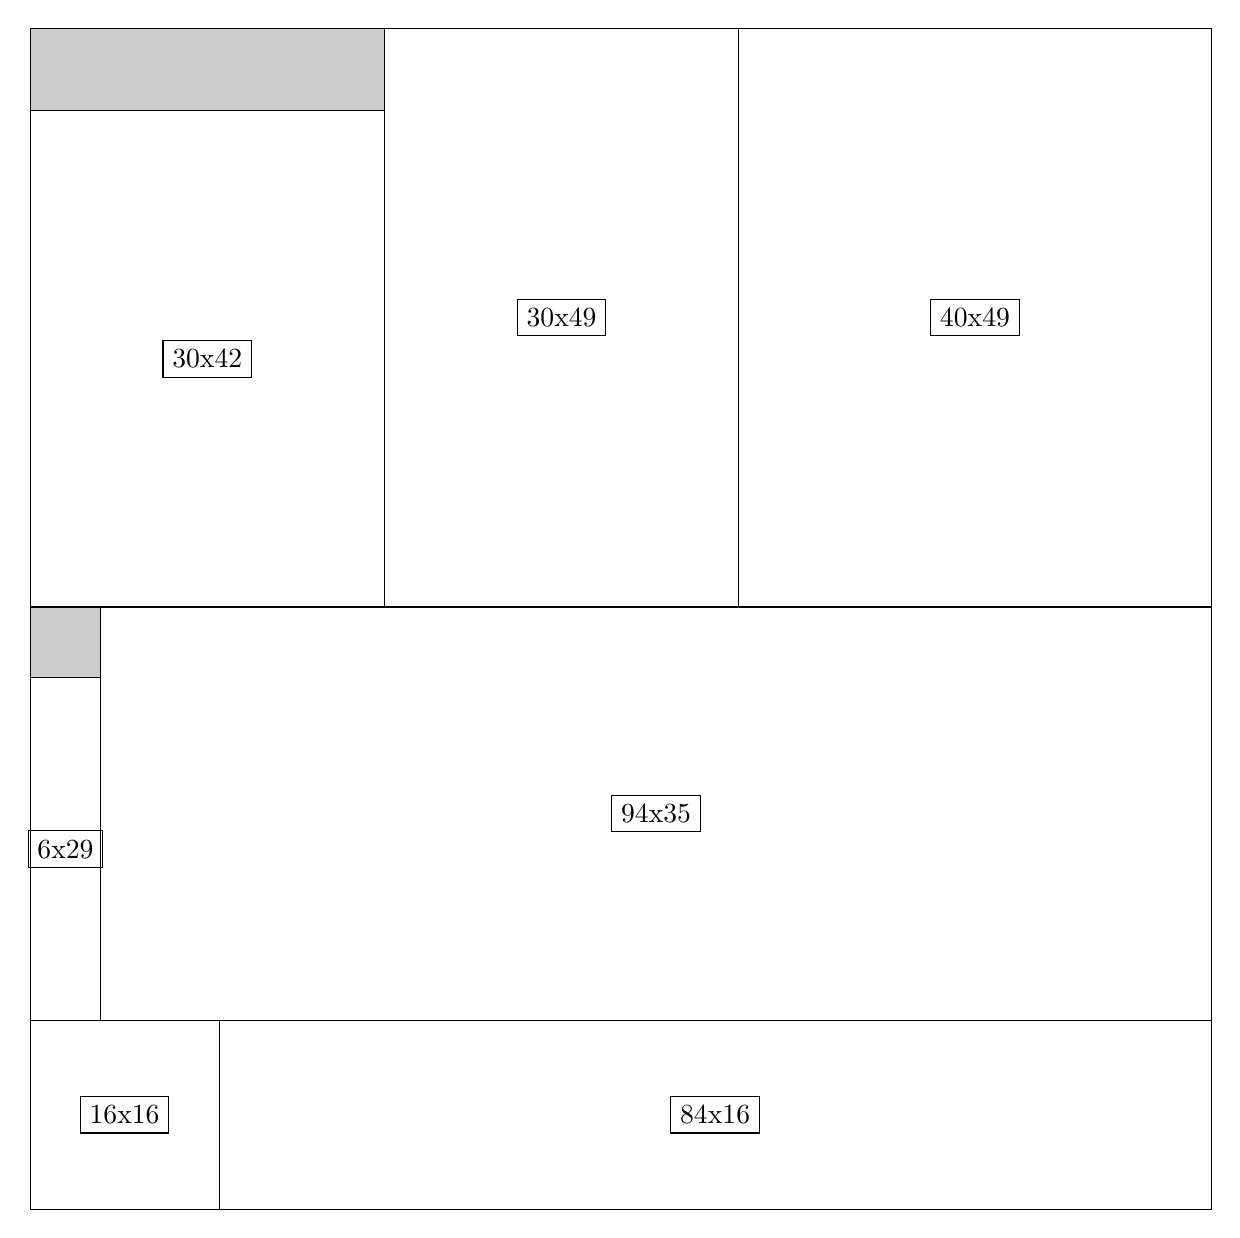
\begin{tikzpicture}[shorten >=1pt,scale=1.0,every node/.style={scale=1.0},->]
\tikzstyle{vertex}=[circle,fill=black!25,minimum size=14pt,inner sep=0pt]
\filldraw[fill=gray!40!white, draw=black] (0,0) rectangle (15.0,15.0);
\foreach \name/\x/\y/\w/\h in {84x16/2.4/0.0/12.6/2.4,16x16/0.0/0.0/2.4/2.4,94x35/0.8999999999999999/2.4/14.1/5.25,6x29/0.0/2.4/0.8999999999999999/4.35,40x49/9.0/7.6499999999999995/6.0/7.35,30x49/4.5/7.6499999999999995/4.5/7.35,30x42/0.0/7.6499999999999995/4.5/6.3}
\filldraw[fill=white!40!white, draw=black] (\x,\y) rectangle node[draw] (\name) {\name} ++(\w,\h);
\end{tikzpicture}


w =84 , h =16 , x =16 , y =0 , v =1344
\par
w =16 , h =16 , x =0 , y =0 , v =256
\par
w =94 , h =35 , x =6 , y =16 , v =3290
\par
w =6 , h =29 , x =0 , y =16 , v =174
\par
w =40 , h =49 , x =60 , y =51 , v =1960
\par
w =30 , h =49 , x =30 , y =51 , v =1470
\par
w =30 , h =42 , x =0 , y =51 , v =1260
\par
\newpage


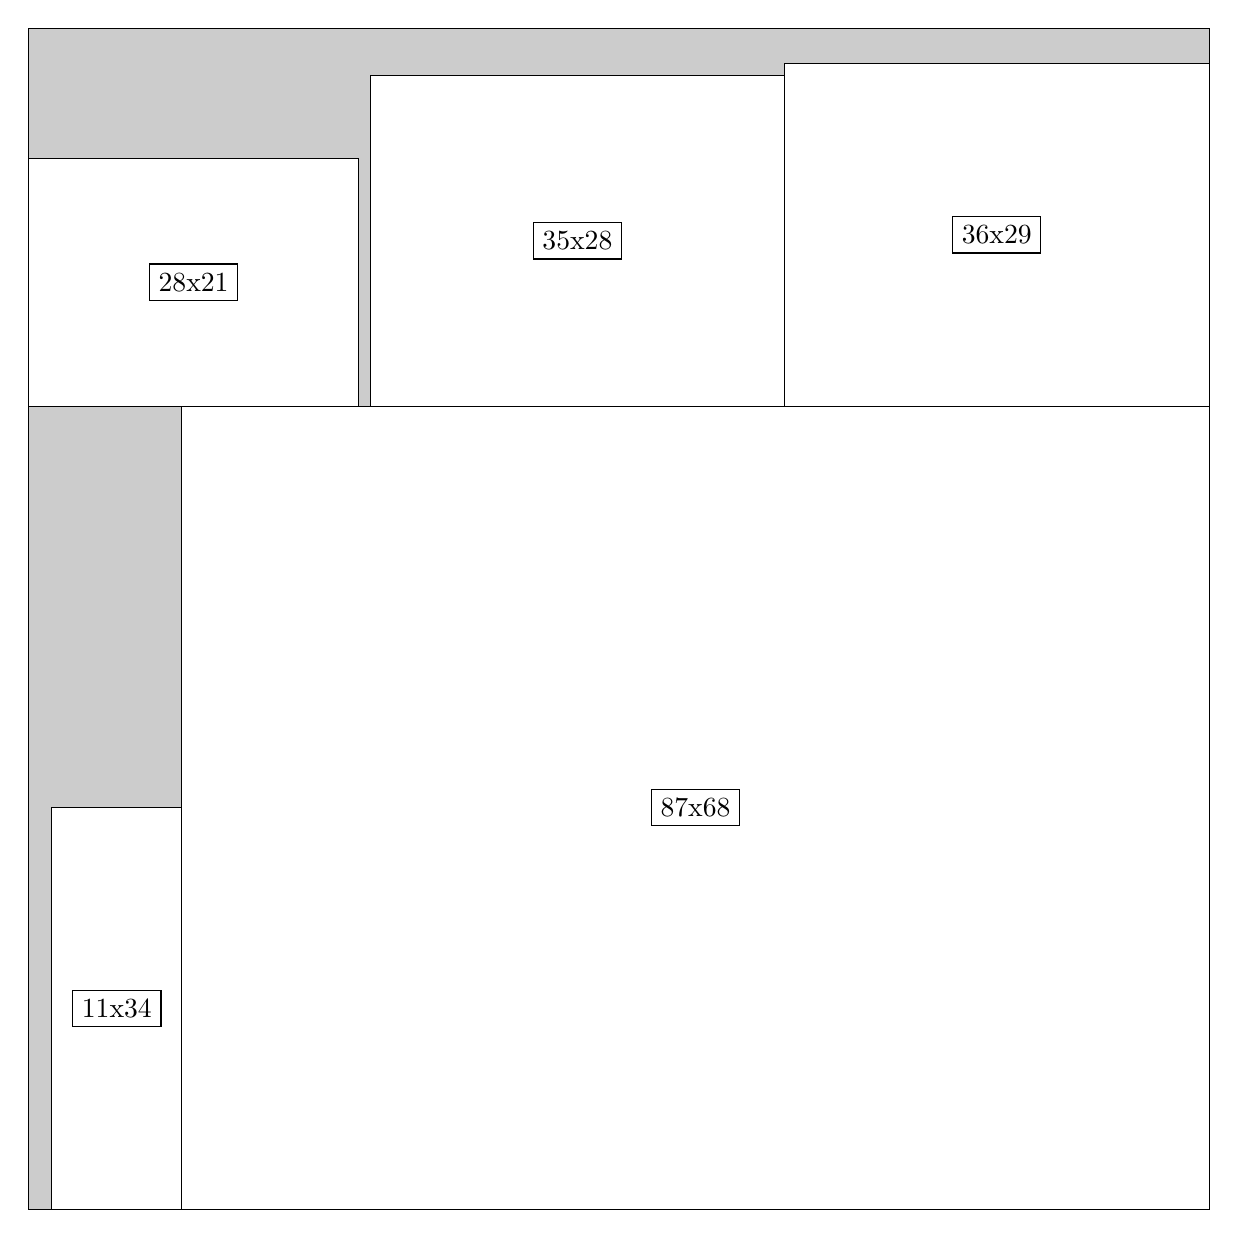
\begin{tikzpicture}[shorten >=1pt,scale=1.0,every node/.style={scale=1.0},->]
\tikzstyle{vertex}=[circle,fill=black!25,minimum size=14pt,inner sep=0pt]
\filldraw[fill=gray!40!white, draw=black] (0,0) rectangle (15.0,15.0);
\foreach \name/\x/\y/\w/\h in {87x68/1.95/0.0/13.049999999999999/10.2,11x34/0.3/0.0/1.65/5.1,36x29/9.6/10.2/5.3999999999999995/4.35,35x28/4.35/10.2/5.25/4.2,28x21/0.0/10.2/4.2/3.15}
\filldraw[fill=white!40!white, draw=black] (\x,\y) rectangle node[draw] (\name) {\name} ++(\w,\h);
\end{tikzpicture}


w =87 , h =68 , x =13 , y =0 , v =5916
\par
w =11 , h =34 , x =2 , y =0 , v =374
\par
w =36 , h =29 , x =64 , y =68 , v =1044
\par
w =35 , h =28 , x =29 , y =68 , v =980
\par
w =28 , h =21 , x =0 , y =68 , v =588
\par
\newpage


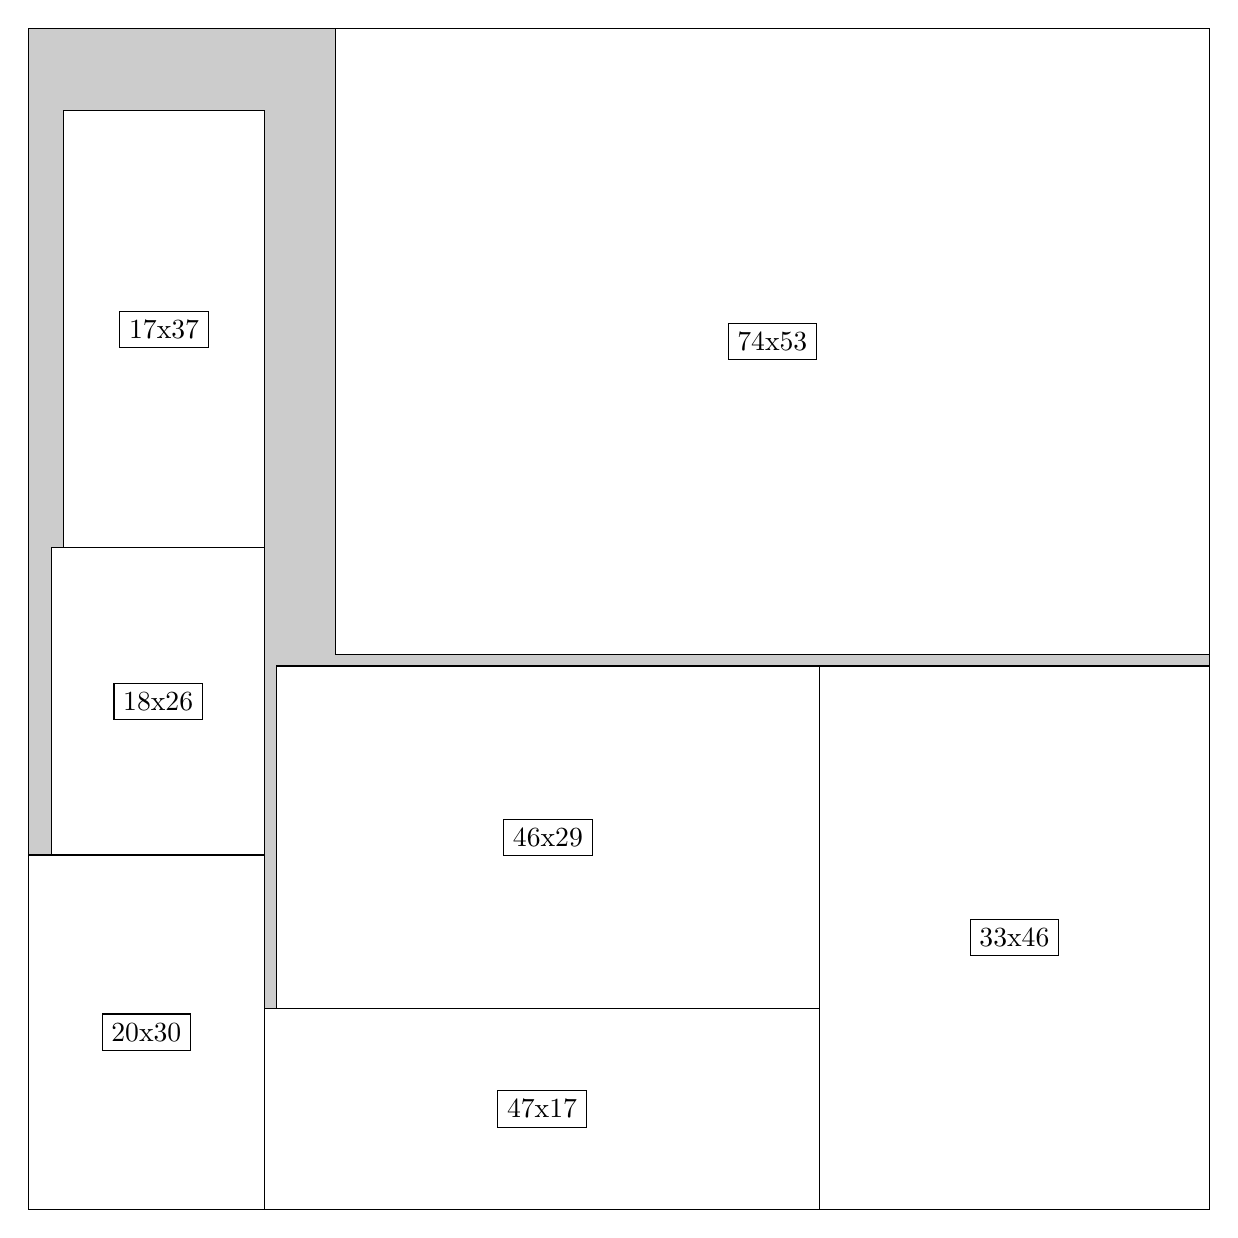
\begin{tikzpicture}[shorten >=1pt,scale=1.0,every node/.style={scale=1.0},->]
\tikzstyle{vertex}=[circle,fill=black!25,minimum size=14pt,inner sep=0pt]
\filldraw[fill=gray!40!white, draw=black] (0,0) rectangle (15.0,15.0);
\foreach \name/\x/\y/\w/\h in {33x46/10.049999999999999/0.0/4.95/6.8999999999999995,47x17/3.0/0.0/7.05/2.55,46x29/3.15/2.55/6.8999999999999995/4.35,74x53/3.9/7.05/11.1/7.949999999999999,20x30/0.0/0.0/3.0/4.5,18x26/0.3/4.5/2.6999999999999997/3.9,17x37/0.44999999999999996/8.4/2.55/5.55}
\filldraw[fill=white!40!white, draw=black] (\x,\y) rectangle node[draw] (\name) {\name} ++(\w,\h);
\end{tikzpicture}


w =33 , h =46 , x =67 , y =0 , v =1518
\par
w =47 , h =17 , x =20 , y =0 , v =799
\par
w =46 , h =29 , x =21 , y =17 , v =1334
\par
w =74 , h =53 , x =26 , y =47 , v =3922
\par
w =20 , h =30 , x =0 , y =0 , v =600
\par
w =18 , h =26 , x =2 , y =30 , v =468
\par
w =17 , h =37 , x =3 , y =56 , v =629
\par
\newpage


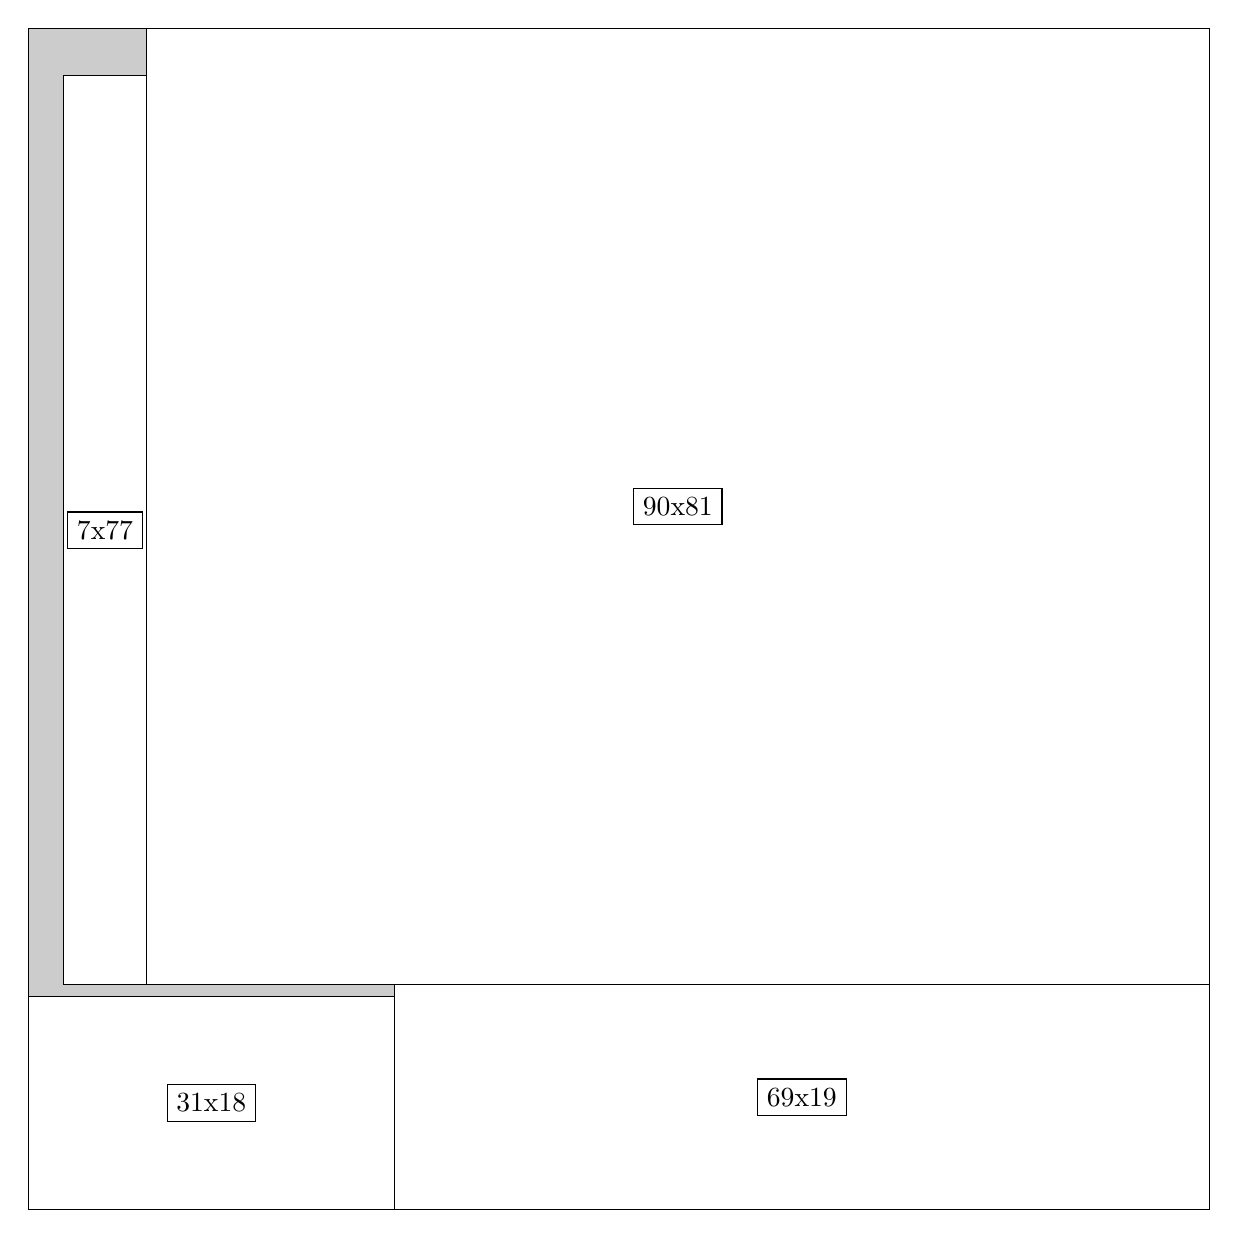
\begin{tikzpicture}[shorten >=1pt,scale=1.0,every node/.style={scale=1.0},->]
\tikzstyle{vertex}=[circle,fill=black!25,minimum size=14pt,inner sep=0pt]
\filldraw[fill=gray!40!white, draw=black] (0,0) rectangle (15.0,15.0);
\foreach \name/\x/\y/\w/\h in {69x19/4.6499999999999995/0.0/10.35/2.85,31x18/0.0/0.0/4.6499999999999995/2.6999999999999997,90x81/1.5/2.85/13.5/12.15,7x77/0.44999999999999996/2.85/1.05/11.549999999999999}
\filldraw[fill=white!40!white, draw=black] (\x,\y) rectangle node[draw] (\name) {\name} ++(\w,\h);
\end{tikzpicture}


w =69 , h =19 , x =31 , y =0 , v =1311
\par
w =31 , h =18 , x =0 , y =0 , v =558
\par
w =90 , h =81 , x =10 , y =19 , v =7290
\par
w =7 , h =77 , x =3 , y =19 , v =539
\par
\newpage


\end{document}